\section{Level 1 Jet Calibration for the High Luminosity LHC}
\label{sec:pu140_calib}
The inputs to the trigger do not exactly represent the offline quantities and the L1 jets have an more rigid size than the simulated Gen jets. By correcting the energy of the L1 jets through calibration it is possible to scale there energy to be closer to that of the Gen jets in an event \cite{l1jet-calibration}. It was necessary to produce a set of calibrations for L1 jets made with simulated data for the High Luminosity upgrade of the LHC, with PU of $\sim140$ per bunch crossing, for studies on the upgrade.
\\\\
To perform the calibration, L1 jets are matched to Gen jets produced from MC truth quantities (required to have $\Delta R<0.3$) for a collection of MC simulated events. For a particular bin of Gen $p_T$, a Gaussian is fit to the distribution of L1 jet $p_T$, giving a mean and its standard deviation. This value is plotted on the $x$ axis of the plot in Fig.~\ref{fig:calibfit}. The $y$ value is found by fitting in the same bin the ratio of the Gen and L1 $p_T$. The result is a set of points that can be fit with an appropriate function. To calibrate L1 jets in the future, the correction factor can be calculated by reading off the value of the fit function at a certain L1 $p_T$. 
\\\\
The performance of this calibration can be seen in Fig.~\ref{fig:calibclosure}. In this case the calibration is effective down to around $30$~GeV. This is expected as the fit was only valid until this value. In high PU samples the low energy L1 jets are heavily contaminated. This results in the Gen jets not being matched to the correct corresponding L1 jet, characterised by the turn over in the ratio as the $p_T$ decreases.
%why calibrate
%calibration theory- fit
\begin{figure}
	\begin{center}
		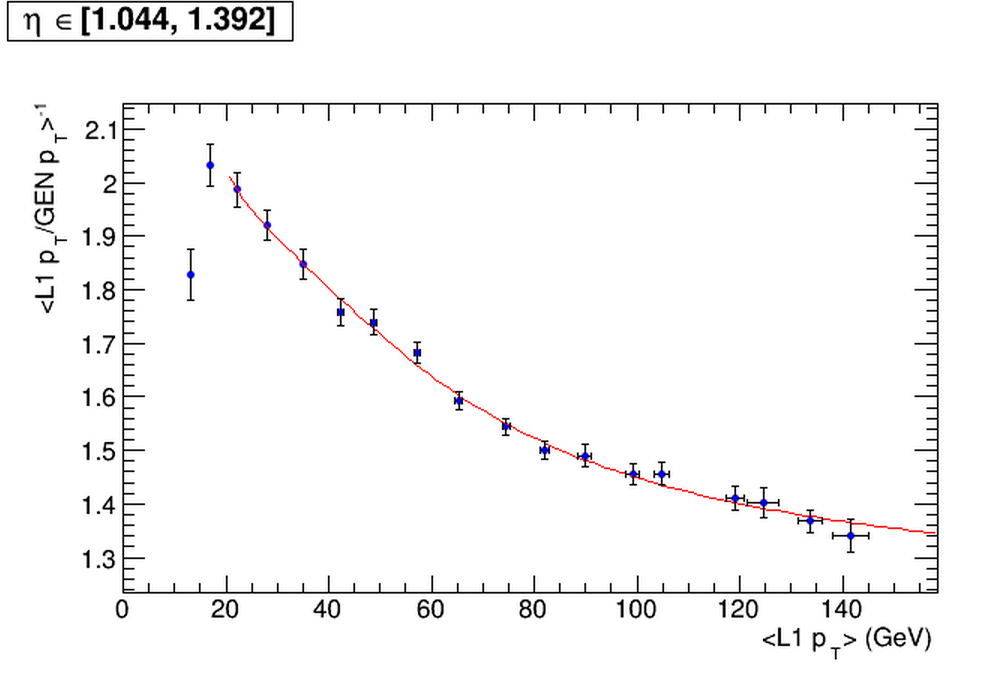
\includegraphics[width=0.6\linewidth]{pu140_calibrationfit}
	\end{center}
	\caption{A fit to the L1 $p_T$ against its ratio with Gen for a particular $\eta$ bin. This fit is used to calculate calibration factors for the L1 jets.}
	\label{fig:calibfit}
\end{figure}
%explain turnover
%closure test- plots
\begin{figure}
	\begin{center}
		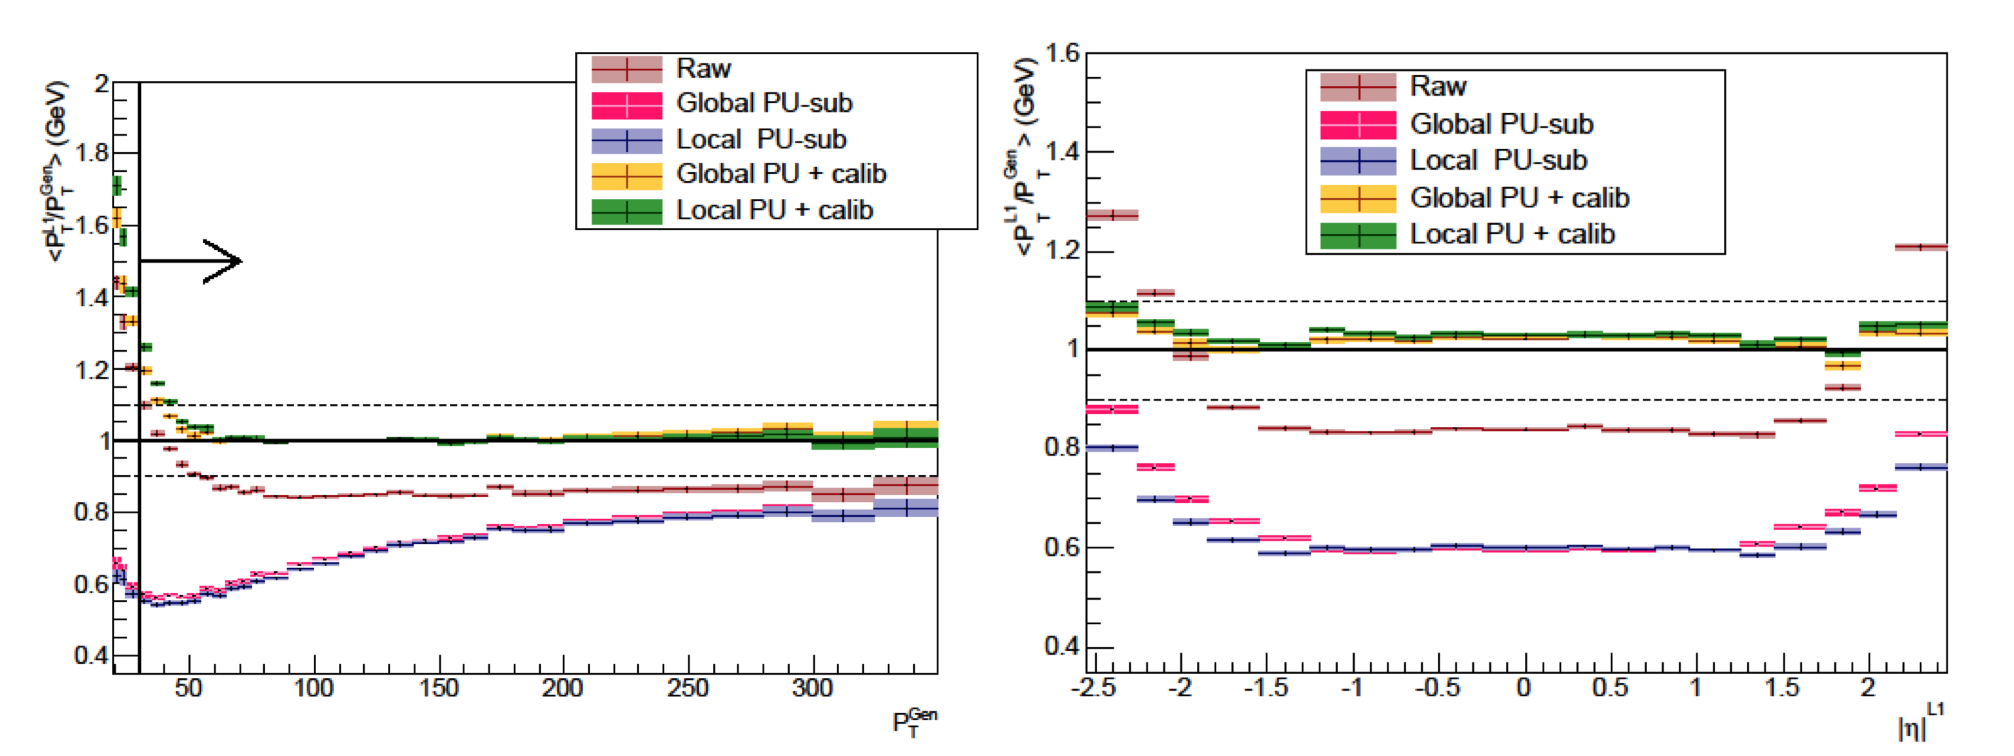
\includegraphics[width=1.0\linewidth]{pu140_calib_closure}
	\end{center}
	\caption{The ratio of L1 jets with Gen before and after they are calibrated, demonstrating the effectiveness of the calibration \cite{nick-pu140calib}}
	\label{fig:calibclosure}
\end{figure}
